\section{Control of energy storage and its applications}
\label{ch-literature:sec:control-of-energy-storage}

Installing BESS at a strategic location in the LV network brings several advantages to DNOs' control over the network's performance.
Regulating voltages to stay within statutory operating bands \cite{Yang2014}, improving power quality by optimising its power factor \cite{Chua2012b}, shaving peak load to relieve stress from the installed network assets \cite{Bennett2015}, or reducing phase unbalance to increase network efficiency \cite{Wang2015b} are only a few examples of recent research in this field.
Whilst the questions regarding locating and scaling of BESS have mostly been addressed, BESS control still remains an open question and can be split into two complementing yet unmarried approaches:

\begin{enumerate}
	\item ``off-line'' control, using load forecasts and BESS schedules; and
	\item ``on-line'' control, using Set-Points Control (SPC), Model Predictive Control (MPC) or similar dynamic control methods.
\end{enumerate}

These two control approaches have evolved from two different fields of active network management.
Nonetheless, both approaches hold significant benefits to the operational performance of power distribution networks and neither of the two can be neglected.
Therefore, Section \ref{ch-literature:subsec:off-line-and-on-line-control} addresses and discusses the two control approaches and their missing link.

The current form of the NTVV project focuses on controlling a single BESS in the LV distribution network.
However, the uptake of household connected BESS will increase the number of distributed systems, which need to be managed cooperatively.
Therefore, Section \ref{ch-literature:subsec:centralised-and-distributed-control} reviews and discusses different control approaches for distributed BESS, since the control of multiple single-phase storage units in a three-phase network is inherently more challenging that controlling a single three-phase device.

\subsection{Off-line and on-line control}
\label{ch-literature:subsec:off-line-and-on-line-control}

Off-line control uses historic data to predict future load patterns, which are used to schedule BESS operation accordingly.
Early approaches, e.g. by Oudalov et al. \cite{Oudalov2007}, who used dynamic programming to generate BESS schedules, had relatively high forecast errors due to the inherent difficulty of predicting future loads.
These errors ultimately limit the ability of any given BESS schedule to e.g. effectively reduce peaks.
This is why recent research begun including uncertainty, like the work done by Baker et al. \cite{Baker2017} where uncertainty of wind power was taken into account when scheduling and sizing BESS.
Other work frequently re-evaluates BESS schedules to control and adjust its schedules after completing individual decision epochs \cite{Wang2014a}.
Nonetheless, load forecasting remain a key component for BESS scheduling despite those load forecasts (and the resulting BESS schedules) being imperfect.
This fact was emphasised by Rowe et al. in \cite{Rowe2014a}, and they developed a filtering mechanism for scheduling algorithms to reduce peak load in LV networks in spite the presence of forecast errors.
They also highlight the fact that most day-ahead load forecast only predict at a temporal resolution down to half-hourly periods.
The reason behind this choice was pointed out by Haben et al. in \cite{Poghosyan2014, Haben2014}, as they argue that forecasts at half-hourly resolution yield the best compromise between high accuracy and high temporal resolution.
Therefore, half-hourly forecasts have become the standard for generating any resource commitment and resource operation schedules.
However, sub-half-hourly load volatility imposes the biggest stress on the network and it is this volatility that cannot be addressed when relying on half-hourly forecast alone.
Therefore, on-line control has been considered as an alternative to off-line control.

One flavour of on-line control is the Set-Point Control (SPC), which is a robust technique that can immediately respond to network changes.
Since this kind of control runs the risk of reaching shortage or surplus of BESS stored energy, modifications like hysteresis control and ramp-rate control were proposed \cite{Gybel2012, Blaabjerg2006, Malesani1990, Xu2011a, Such2012}.
In \cite{Such2012}, Such and Hill showed how a ramp controlled BESS could smoothen the volatile power from wind generation.
Furthermore, their work shows how reverse power flow can be completely omitted through the use of on-line BESS control.
However, this kind of on-line control is less effective in addressing daily demand peaks, since pure SPC can only react to present network demand and does not respond to general trends or upcoming load events.
Also, incorrect set-point thresholds of insufficient network impact can also lead to an excess or shortage in BESS supply, which is shown in the example Figure \ref{ch-literature:fig:spc}.

\begin{figure}\centering
	\subfloat[]{
		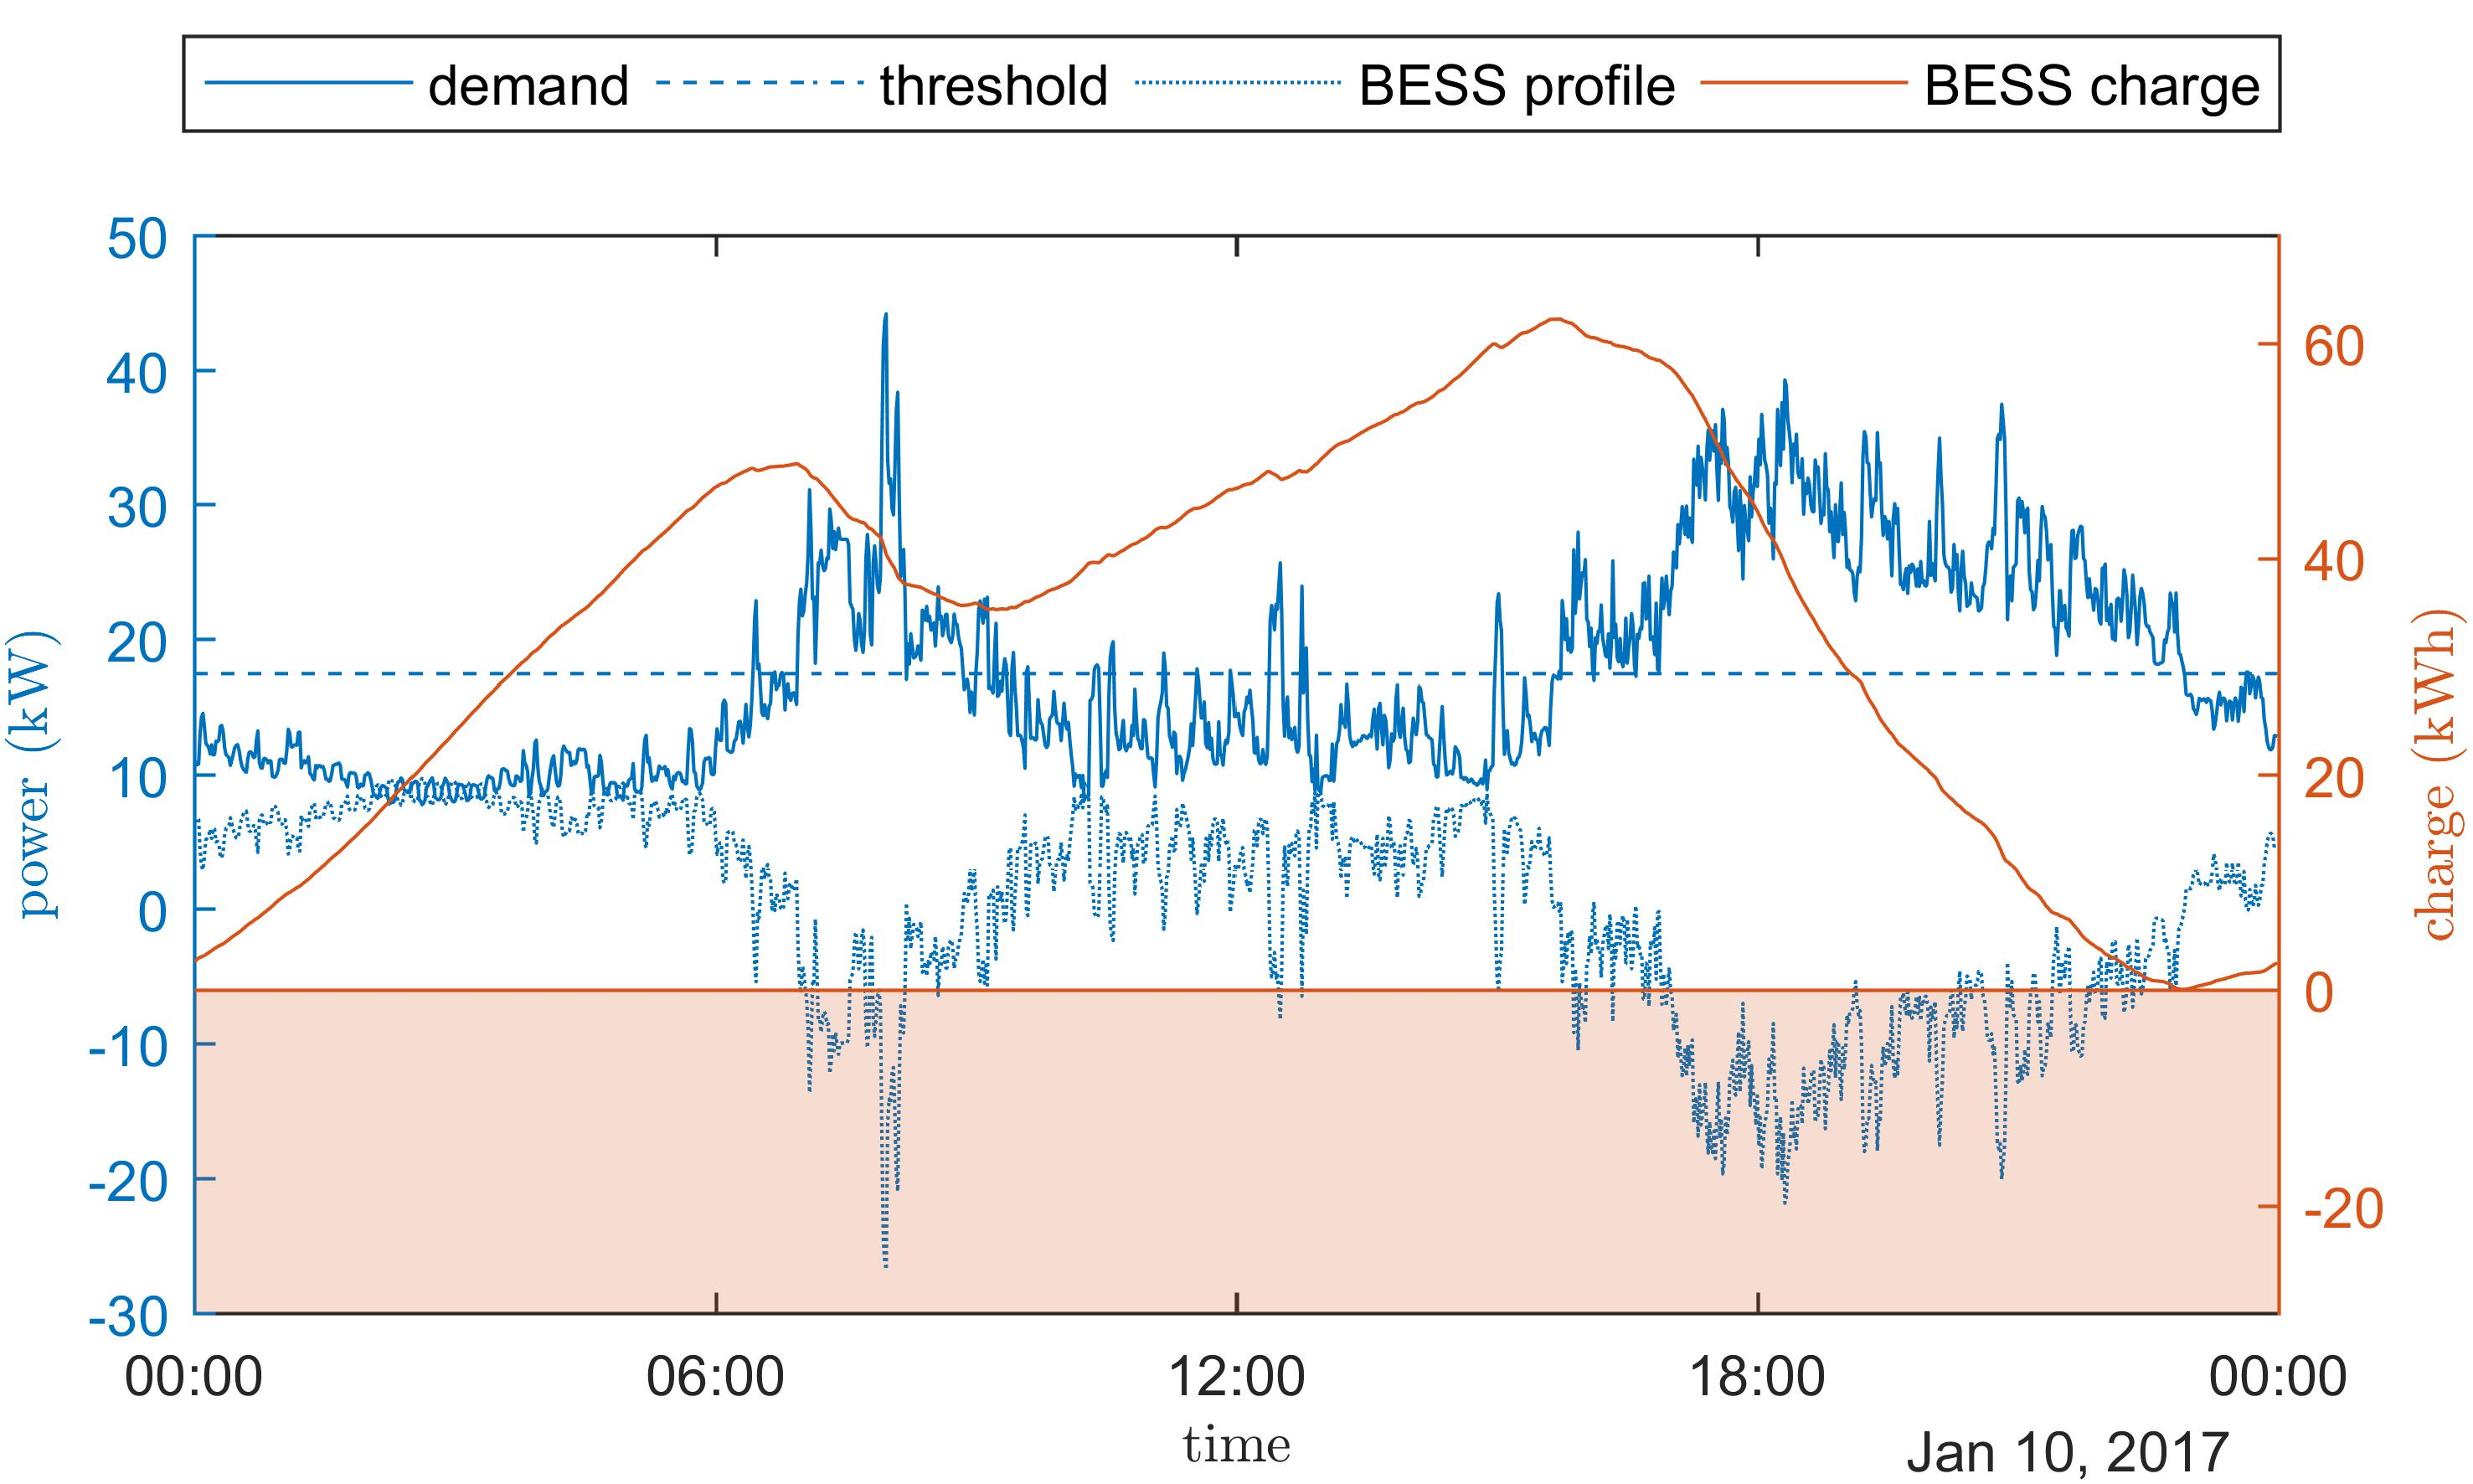
\includegraphics{_literature/fig/spc-failure-ok}
		\label{ch-literature:subfig:spc-ok}
	}\\
	\subfloat[]{
		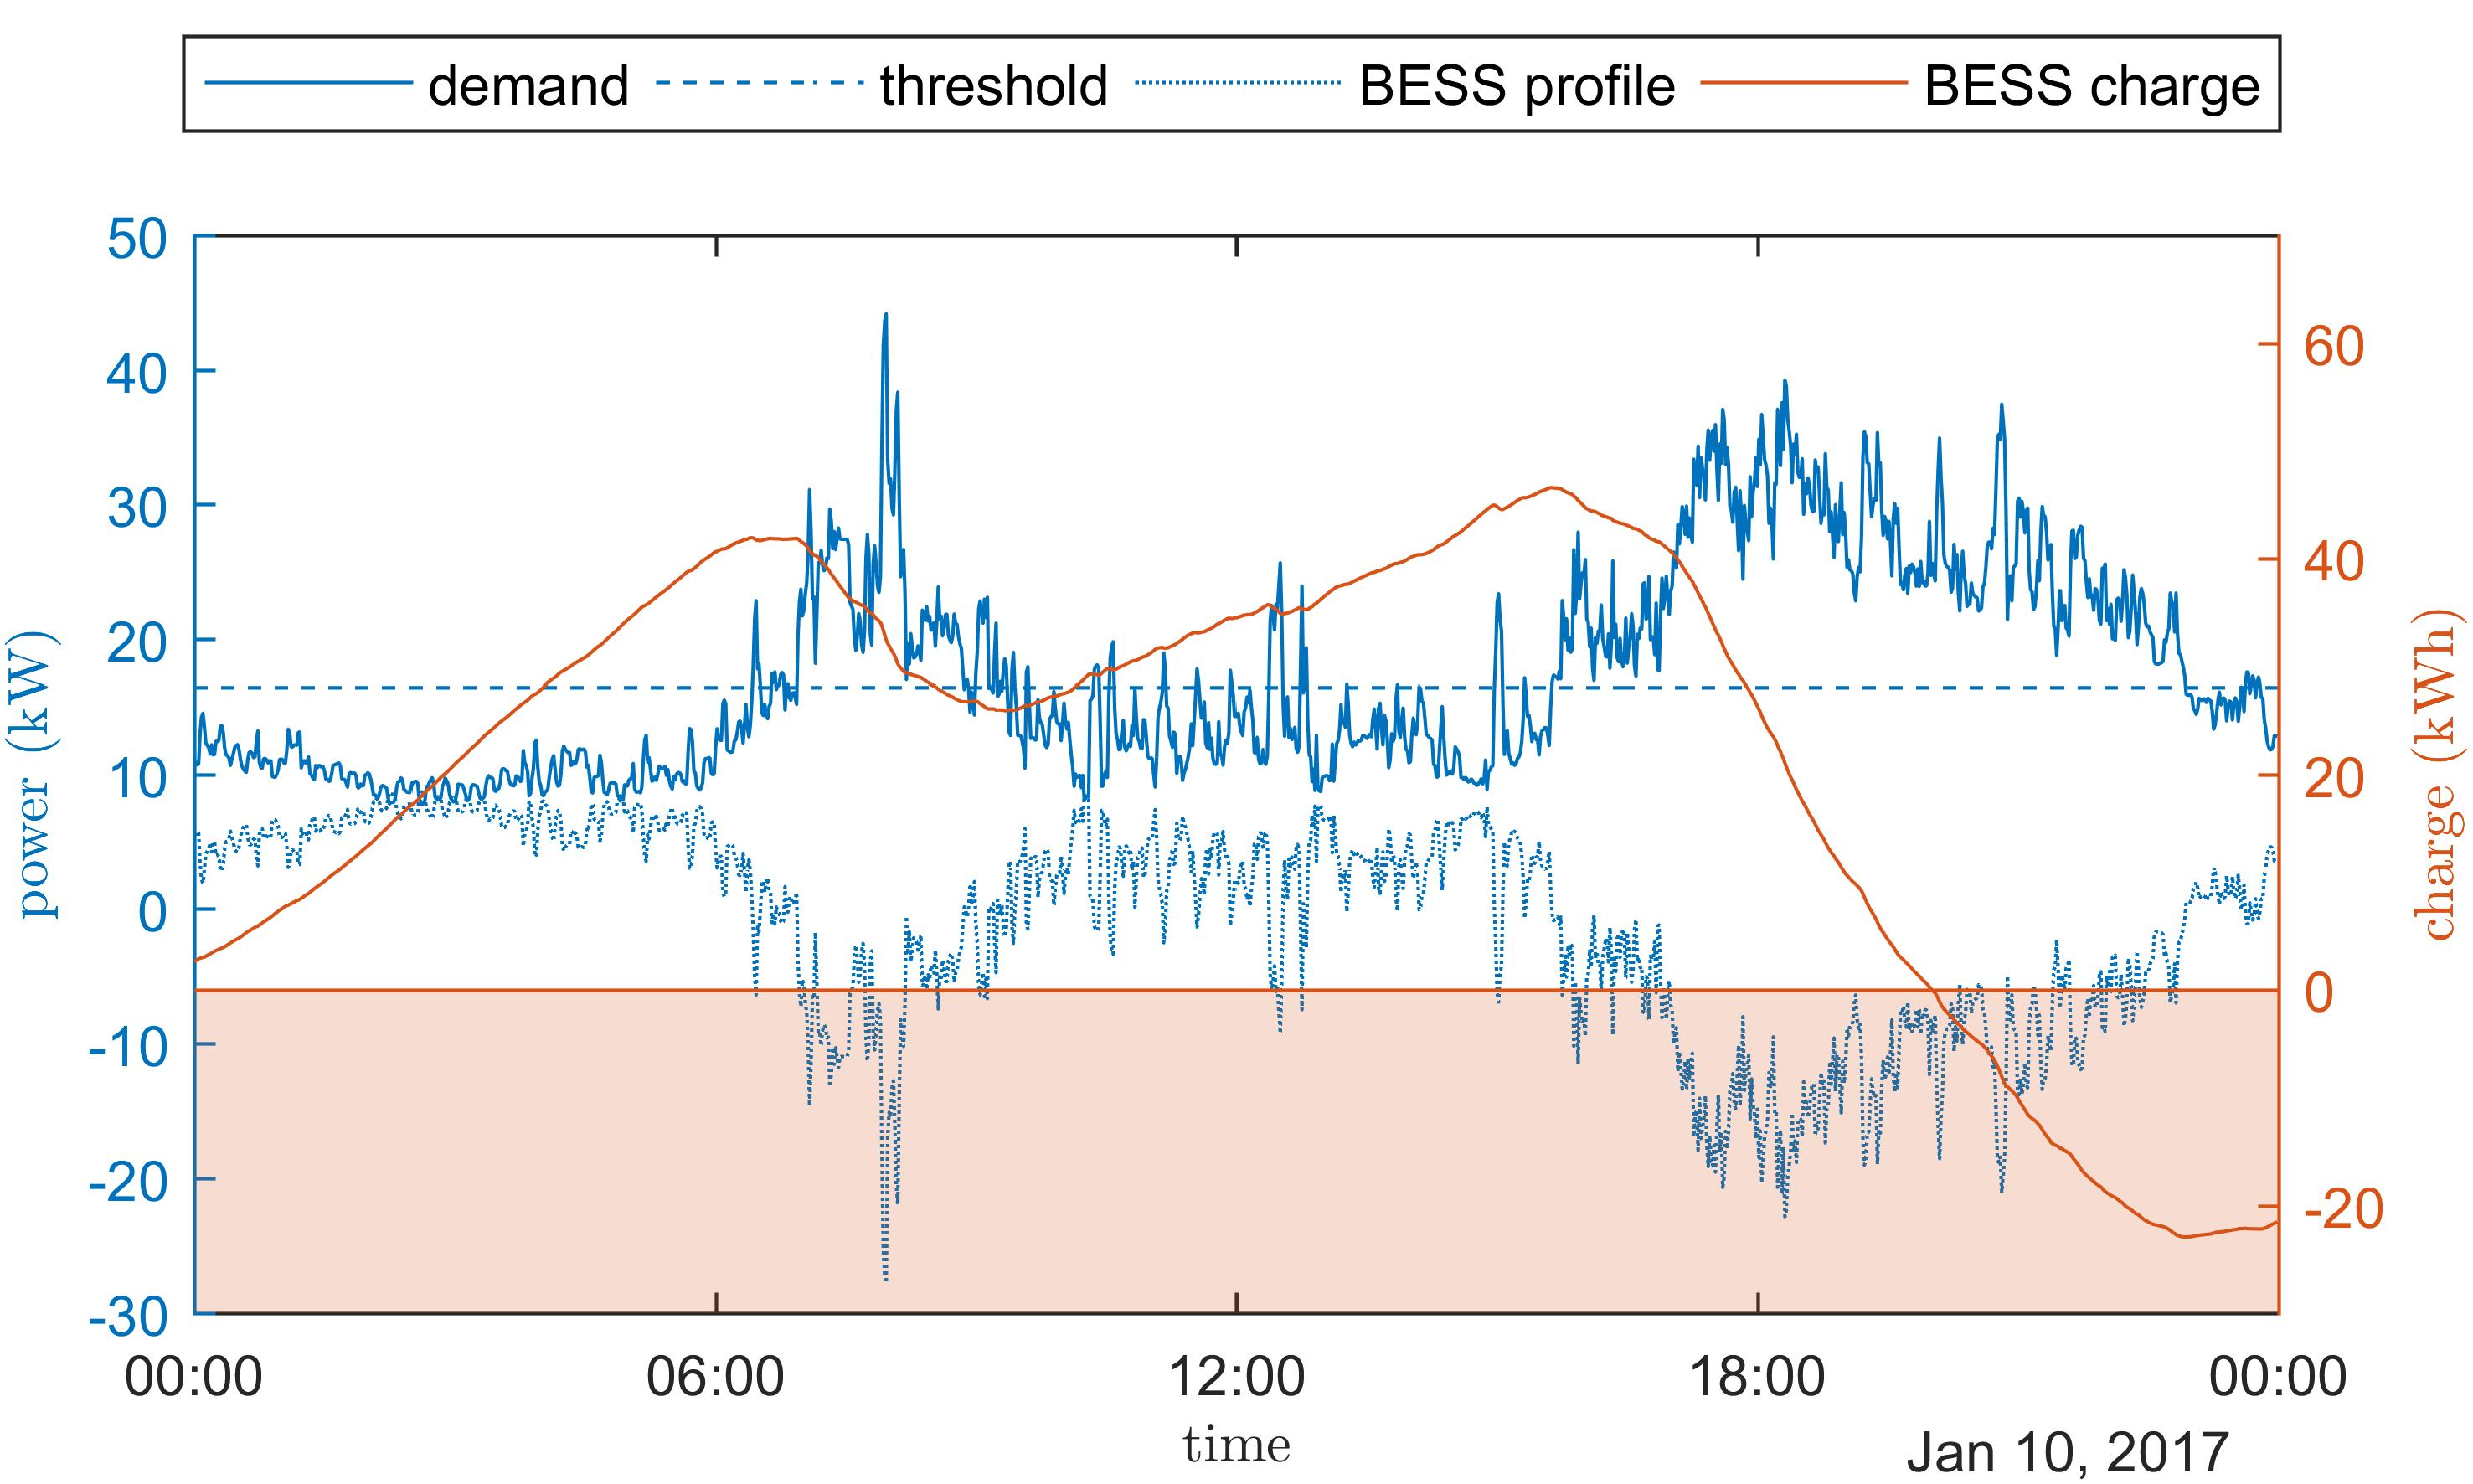
\includegraphics{_literature/fig/spc-failure-bad}
		\label{ch-literature:subfig:spc-bad}
	}
	\caption{An example of a set-point controlled BESS to show a potential shortage of storage capacity when choosing the controlling threshold incorrectly: (a) with correctly chosen threshold, and (b) incorrectly chosen threshold.}
	\label{ch-literature:fig:spc}
\end{figure}

In the example in Figure \ref{ch-literature:fig:spc}, a BESS is operated to compensate for demand fluctuations.
The top figure (Fig. \ref{ch-literature:subfig:spc-ok}) represents the BESS operation when the SPC threshold is perfectly chosen.
The top figure (Fig. \ref{ch-literature:subfig:spc-bad}) shows the same operation but with a SPC threshold deviation of 1kW.
In the latter scenario, BESS experiences a shortage of supply at peak demand time (zero-crossing arund 20:00), which would prevent the device from supplying its peak-shaving functions.
In order to address these shortcomings SPC has been extended by using short-term load predictions through the implementation of Model Predictive Control (MPC).
Some MPC examples include Auto-Regressive (AR) models \cite{Li2009, Nie2011}, fuzzy logic models \cite{Sannomiya2001, Chen2013a}, genetic algorithms \cite{Xia2015a, Liu2015} or Artificial Neural Networks (ANN) \cite{Kalogirou2014, Quan2014, Lee2014, Pezeshki2014, Vaz2016, Reihani2016, Xiao2017}.
The increasing complexity of MPC yields a better prediction performance.
For instance, Reihani et al. in \cite{Reihani2016} use the most recent 20 minutes of load information with a complex-valued ANN to predict the next 20 minutes of minutely load variations.
Since their raw forecasts were more erratic than the actual load profile, a Kalman filter was implemented to smoothen the MPC's output, yet this step introduced significant discrepancies between the actual and the forecasted load.
Therefore, they increased MPC complexity even further by taking into account parallel time-series, i.e. they considered the same 20 minutes from previous days in the prediction mechanism.
This addition produced significantly better results and they shaved daily peaks by around 300kW.
Implementing such increasingly complex MPC to support on-line control is therefore a promising research trend, however the computational burden to deliver real-time solutions makes implementation of such systems not yet feasible.

Finding a way of combining both scheduled BESS operation, which is executed at half-hourly resolution, with a responsive correction mechanism is therefore an open research question that has not yet been addressed.
Objectives 1 and 2, as outlined in Section \ref{ch-introduction:sec:problem-statement}, and their corresponding chapters, respectively Chapter \ref{ch1} and Chapter \ref{ch2}, address this question in two ways.
First, by assessing the ability to apply scheduled BESS operation onto a three-phase network in a sub-half-hourly manner, yet without modifying its underlying half-hourly schedule.
Then, the scheduling constraint is lifted by allowing an operational tolerance in order.

\subsection{Centralised and distributed control}
\label{ch-literature:subsec:centralised-and-distributed-control}

The monitoring and control of any distributed system, and hence of any power network, includes four systems that are inherently linked \cite{Mansouri-Samani1993}:

\begin{enumerate}
	\item The \textit{managed system} itself, i.e. power network, that needs to be controlled;
	\item a \textit{monitoring system} that generates data through sensors and measuring equipment that is installed in the \textit{managed system};
	\item a \textit{decision making system} that uses the provided data to generate certain aims, e.g. to improve the system state; and
	\item a \textit{control system} to generate control actions for the \textit{managed system}.
\end{enumerate}

\nomenclature[G]{IoT}{Internet of Things}
\nomenclature[G]{SCADA}{Supervisory Control And Data Acquisition}

In traditional power system control, systems 1 and 2 are grouped into the distributed measuring system and systems 3 and 4 are grouped into a centralised controller \cite{Nelson1985}.
Therefore, a bidirectional flow of information had to exist in order to control and assure operation of the underlying physical network.
Supervisory Control And Data Acquisition (SCADA) is the typical control architecture that enables the implementation of this bidirectional information flow.
Tokyo is a showcase of implementing such a centralised control system.
In 1990, \textit{Tokyo Electric Power Co.} (TEPCO) and \textit{Toshiba} presented their latest installation of a centrally managed power distribution network that could deliver 43GW of power to the entire city of Tokyo.
All control instructions were generated from TEPCO's central dispatching centre, which took into account measurements from a network of 819 nodes and 938 branches.
Since Tokyo has grown significantly over the past decades, computational burden to relay data and act upon the information has increased, too.
The UK power network is also a centrally managed system that has seen an increase in complexity, yet ``\textit{the network is 99.9999\% reliable - a statistic we're proud of}``\cite{NationalGrid2017}.


\nomenclature[G]{FIPA}{Foundation for Intelligent Physical Agents}
\nomenclature[G]{ITC}{Information and Communication Technology}

But with the deployment of smart meters, network enabled appliances and controllable LCTs that can be part of the a so called ``Internet of Things'' (IoT), system complexity is expected to increase beyond the capabilities of a single central management centre, which is why research begun focusing on distributed control mechanisms \cite{Vovos2007, Guerrero2008, Bidram2014, Sugihara2013, Toledo2013, Marra2013, Mokhtari2013, Gill2014, Dolan2012, Atia2016, Bidram2012, Wang2016}.
In fact, in the majority of existing literature that uses BESS in distribution networks focuses on voltage security \cite{Sugihara2013, Toledo2013, Marra2013, Mokhtari2013, Atia2016}, power flow management \cite{Guerrero2008, Wang2016} and management of flexible loads \cite{Gill2014, Dolan2012}.
For instance, the approach used by Mokhtari et al. in \cite{Mokhtari2013} relies on bus voltage and network load measurements to prevent system overloads, and Marra et al. in \cite{Marra2013} go even further and use information sharing between PV and BESS in order to limit voltage deviation.
Both research teams were able to stabilise the network, and Marras et al. even increased the voltage margin by an additional 6.1V.
The reasons why the usage of distributed and hierarchical control systems have become this attractive include lighter computational load for all control systems through abstraction at higher control levels and improved system stability, security and redundancy \cite{Guerrero2013, Guerrero2013a}.

Approaches and topologies to manage the flow of information within these control systems are classified by Bidram et al. in \cite{Bidram2014}, where they separate the real network, i.e. the \textit{physical layer}, from Information and Communication Technology (ITC), i.e. the \textit{cyber communication layer}.
This separation allowed them to represent any distributed power system as a system of multiple cooperating entities, i.e. intelligent agents that form a so called Multi-Agent System (MAS).
The technology of MAS comes from computer science and is well established in theory and practice of intelligent agents \cite{Russell2009}.
As stated by Wooldridge et al. in \cite{Wooldridge1995}, intelligent agents are flexible and autonomous entities that are defined by three fundamental properties:

\begin{enumerate}
	\item \textit{Reactivity}, which allows an agent to respond to changes in its observed environment,
	\item \textit{Pro-activeness}, which makes an agent act to meet its own or a collaborative goal, and
	\item \textit{Social-ability}, which enables the agent to coordinate its action with other agents.
\end{enumerate}

Computer scientists would describe an agents as a component that gathers and collaboratively reacts to information about its environment, but distributed control systems in power distribution networks share the same characteristics.
For this very reason has MAS seen increasing attention in the power and energy engineering discipline, where the agents' goals were focusing on integration of DERs \cite{Al-Hinai2004, Dimeas2005, Vasirani2013, Dou2017, Gomez-Sanz2014}, matching of demand and supply \cite{Kok2005}, restoring the power distribution network \cite{Li2012}, reconfiguring the network to reduce unbalance \cite{Ding2016}, integration of EVs \cite{Lopez2011, Karfopoulos2013, Ramachandran2013, GrauUnda2014} and providing voltage support \cite{Baran2007}.
Standardisation across MAS was established by the Foundation for Intelligent Physical Agents (FIPA), yet as explored by Catterson et al. in \cite{Catterson2005}, the underlying versatility of different MAS makes integration very challenging.
Also, as the number of independent elements becomes ubiquitous, requirements for a strong telecommunications infrastructure become equally important \cite{Hatziargyriou2015}.
So far, synchronisation amongst agents has been taken for granted, yet MAS on multilayer networks may not automatically be synchronised \cite{He2017}.
Assessing the impact of introducing such a desynchronisation has therefore become part of the research that is presented in this thesis.
Objective 3, as outlined in Section \ref{ch-introduction:sec:problem-statement}, addresses this research question by subjecting a smart charging algorithm to both a synchronised and a desynchronised MAS environment.

\subsection{Communication-less control}
\label{ch-literature:subsec:communication-less-control}

Another method of implementing a distributed system is to not use any kind of communications infrastructure, since this infrastructure may not always be installed despite being a common assumption when controlling distributed BESS \cite{Hatziargyriou2015}.
Such communication-less systems are typically collections of multiple ``dumb'' devices that follow their own control instructions without any external inputs.
The current procedure of charging EVs is a perfect example of such a system, since their charging commences immediately after they have been plugged into the grid.
At the current rate of EV uptake, which is anticipated to increase with improved driving range, reduced cost of purchase and greater emphasis on leading an environmentally-friendly lifestyle \cite{Shah2015}, so called ``dumb charging'' (or any ``dumb action'' for that matter) has high potential of causing significant network issues \cite{Hota2014, Liu2015a}; i.e. voltage deviations, equipment overloads, asset damage and system outages.
The already mentioned ICT reliant distributed control methods aim to circumvent these issues, using Demand Side Management (DSM) strategies that are based on e.g. game theory \cite{Mohsenian-Rad2010}, time-of-use tariffs \cite{Deilami2011, Surles2012}, or other pricing signals \cite{Masoum2015}.
Without ICT however, none of them can be implemented and instead an indirect method must be sought.

\nomenclature[G]{AIMD}{Additive Increase Multiplicative Decrease}
\nomenclature[G]{V2G}{Vehicle to Grid}

A communication-less form of controlling Distributed Energy Resources (DERs) is the already mentioned Set-Point Control (SPC) \cite{Leadbetter2012}.
Using traditional SPC on multiple identically-configured DERs can provice an optimal operation conditions, if each DER's control parameters (e.g., bus voltage) were shared \cite{Thieblemont2017a}.
But in a communication-less environment this requirement cannot be satisfied, which is why DER control algorithms have to be improved to prevent, for example, devices located furthest from the substation from being used more frequently than others.
The algorithm to be improved for controlling several BESS in a LV network is the Additive Increase Multiplicative Decrease (AIMD) algorithm.
Unlike traditional SPC or hysteresis control like in \cite{Jiang2007}, where a fuel-cell's bus voltage was used as input to a ramp control for active power sharing, AIMD (like MAS) has its roots in computer science.
Originally, AIMD algorithms were applied to congestion management in communications networks using the TCP protocol \cite{Chiu1989}, to maximise utilisation while ensuring a fair allocation of data throughput amongst a number of competing users \cite{Wirth2014}.
The same AIMD-type algorithms have previously been applied to power sharing scenarios in low voltage distribution networks, where the limited resource is the availability of power from the substation's transformer.
One of the first proposed implementations for DER management was by St{\"{u}}dli et al. \cite{Studli2012}, yet their system still required a one-way communications infrastructure to broadcast a ``capacity event'' \cite{Studli2014, Studli2014a}.
Later, their work was extended to include Vehicle to Grid (V2G) applications with reactive power support \cite {Studli2015}, but this work relied on an ITC infrastructure, too.

To not impose additional requirements onto consumer devices, and instead maximise the utility of energy storage, an improved AIMD algorithm with individually tuned control parameters is proposed as part of the research in this thesis.
%As stated by Thieblemont et al. in \cite{Thieblemont2017a}: ``\textit{Energy storage systems play a crucial role in decreasing building energy consumption during peak periods and expanding the use of renewable energies in buildings and communities}''.
Previous research is therefore extended by the presented work, since previous work has only utilised common SPC thresholds for controlling each of the DERs or relied on some form of communications infrastructure.
By proposing an approach to ensure that unavoidable voltage drops along the feeder do not skew the control decisions, and by taking the into consideration voltage oscillations that are caused by demand variation, objective 4, as outlined in Section \ref{ch-introduction:sec:problem-statement}, is addressed.
In strong contrast to the previous work where substation monitoring was used, the proposed AIMD+ algorithm does not require this information, and hence does not require such an extensive communications infrastructure.
